\newpage
\section{Week 3}
\section*{Logistic Regression}
Now we are switching from regression problems to {\bf classification problems}. Don't be confused by the name ``Logistic Regression"; it is named that way for historical reasons and is actually an approach to classification problems, not regression problems.
\section*{Binary Classification}
Instead of our output vector y being a continuous range of values, it will only be 0 or 1.
\[y \in \{0,1\} \]
Where 0 is usually taken as the ``negative class" and 1 as the "positive class", but you are free to assign any representation to it.

We're only doing two classes for now, called a ``Binary Classification Problem."

One method is to use linear regression and map all predictions greater than 0.5 as a 1 and all less than 0.5 as a 0. This method doesn't work well because classification is not actually a linear function.

Hypothesis Representation

Our hypothesis should satisfy:
\[0 \leq h_\theta (x) \leq 1 \]

Our new form uses the {\bf ``Sigmoid Function"}, also called the {\bf ``Logistic Function"}:
\begin{align}
h_\theta (x) &=  g ( \theta^T x ) \\
z &= \theta^T x \\
g(z) &= \dfrac{1}{1 + e^{-z}}
\end{align}

\begin{figure}[ht]
\center
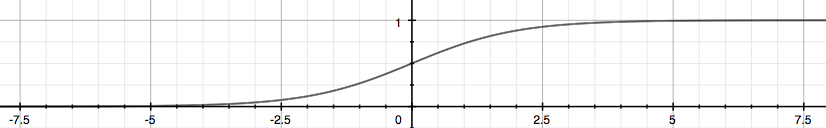
\includegraphics[scale=0.5]{W3_sigmoid}
\caption{Sigmoid Function}
\label{fig:W3_sigmoid}
\end{figure}

The function g(z), shown here, maps any real number to the (0, 1) interval, making it useful for transforming an arbitrary-valued function into a function better suited for classification. Try playing with interactive plot of sigmoid function: \href{https://www.desmos.com/calculator/bgontvxotm}{click here!}.

We start with our old hypothesis (linear regression), except that we want to restrict the range to 0 and 1. This is accomplished by plugging $\theta^T $ into the Logistic Function.

$h_\theta $ will give us the probability that our output is 1. For example, $h_\theta(x)=0.7$ gives us the probability of 70\% that our output is 1.

\begin{align*}
&h_\theta(x) = P(y=1 | x ; \theta) = 1 - P(y=0 | x ; \theta) \\ 
&P(y = 0 | x;\theta) + P(y = 1 | x ; \theta) = 1
\end{align*}

Our probability that our prediction is 0 is just the complement of our probability that it is 1 (e.g. if probability that it is 1 is 70\%, then the probability that it is 0 is 30\%).
\section*{Decision Boundary}
In order to get our discrete 0 or 1 classification, we can translate the output of the hypothesis function as follows:
\begin{align*}
& h_\theta(x) \geq 0.5 \rightarrow y = 1 \\
& h_\theta(x) < 0.5 \rightarrow y = 0 \\
\end{align*}
The way our logistic function g behaves is that when its input is greater than or equal to zero, its output is greater than or equal to 0.5:
\begin{align*}
g(z) \geq 0.5 \\
\text{when } z \geq 0
\end{align*}
Remember:
\begin{align*}
z=0,  e^{0}=1 \Rightarrow  g(z)=1/2\\ 
z \to \infty, e^{-\infty} \to 0 \Rightarrow g(z)=1 \\ 
z \to -\infty, e^{\infty}\to \infty \Rightarrow g(z)=0 
\end{align*}

So if our input to g is $\theta^T$, then that means:
\begin{align*}
& h_\theta(x) = g(\theta^T x) \geq 0.5 \\
& \text{when} \; \theta^T x \geq 0
\end{align*}

From these statements we can now say:
\begin{align*}
& \theta^T x \geq 0 \Rightarrow y = 1 \\
& \theta^T x < 0 \Rightarrow y = 0 \\
\end{align*}

The {\bf decision boundary} is the line that separates the area where y = 0 and where y = 1. It is created by our hypothesis function.

Example:
\begin{align*}
& \theta = 
\begin{bmatrix}
5 \\ 
-1 \\ 
0
\end{bmatrix} \\ 
& y = 1 \; if \; 5 + (-1) x_1 + 0 x_2 \geq 0 \\ 
& 5 - x_1 \geq 0 \\ 
& - x_1 \geq -5 \\
& x_1 \leq 5 \\ 
\end{align*}

In this case, our decision boundary is a straight vertical line placed on the graph where $x_1 = 5$, and everything to the left of that denotes y = 1, while everything to the right denotes y = 0.

Again, the input to the sigmoid function g(z) (e.g. $\theta^T X$) doesn't need to be linear, and could be a function that describes a circle (e.g.$ z = \theta_0 + \theta_1 x_1^2 +\theta_2 x_2^2$) or any shape to fit our data.

\section*{Cost Function}
We cannot use the same cost function that we use for linear regression because the Logistic Function will cause the output to be wavy, causing many local optima. In other words, it will not be a convex function.

Instead, our cost function for logistic regression looks like:
\begin{equation}
J(\theta) = \dfrac{1}{m} \sum_{i=1}^m \mathrm{Cost}(h_\theta(x^{(i)}),y^{(i)})
\end{equation}

\begin{align*}
\mathrm{Cost}(h_\theta(x),y) &= -\log(h_\theta(x)) \; \quad& \text{if y = 1} \\ 
\mathrm{Cost}(h_\theta(x),y) &= -\log(1-h_\theta(x)) \; \quad& \text{if y = 0}
\end{align*}

\begin{figure}[ht]
\center
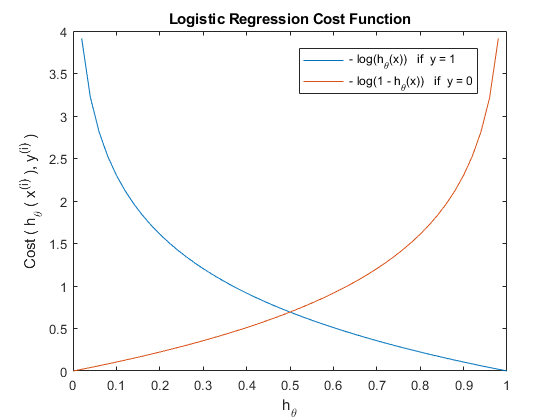
\includegraphics[scale=0.7]{W3_costlogistic}
\caption{Logistic Regression Cost Function}
\label{fig:W3_cost}
\end{figure}

The more our hypothesis is off from y, the larger the cost function output. If our hypothesis is equal to y, then our cost is 0:
\begin{align*}
& \mathrm{Cost}(h_\theta(x),y) = 0 \text{  if  } h_\theta(x) = y \\ 
& \mathrm{Cost}(h_\theta(x),y) \rightarrow \infty \text{  if  } y = 0 \; \mathrm{and} \; h_\theta(x) \rightarrow 1 \\ 
& \mathrm{Cost}(h_\theta(x),y) \rightarrow \infty \text{  if  } y = 1 \; \mathrm{and} \; h_\theta(x) \rightarrow 0 \\ 
\end{align*}
If our correct answer `y' is 0, then the cost function will be 0 if our hypothesis function also outputs 0. If our hypothesis approaches 1, then the cost function will approach infinity.

If our correct answer `y' is 1, then the cost function will be 0 if our hypothesis function outputs 1. If our hypothesis approaches 0, then the cost function will approach infinity.

Note that writing the cost function in this way guarantees that $J(\theta)$ is convex for logistic regression.

\section*{Simplified Cost Function and Gradient Descent}
We can compress our cost function's two conditional cases into one case:

\begin{equation}
\mathrm{Cost}(h_\theta(x),y) = - y \; \log(h_\theta(x)) - (1 - y) \log(1 - h_\theta(x))
\end{equation}

Notice that when y is equal to 1, then the second term $(1-y)\log(1-h_\theta(x))$ will be zero and will not affect the result. If y is equal to 0, then the first term $-y \log(h_\theta(x))$ will be zero and will not affect the result.

We can fully write out our entire cost function as follows:

\begin{equation}
J(\theta) = - \frac{1}{m} \displaystyle \sum_{i=1}^m [y^{(i)}\log (h_\theta (x^{(i)})) + (1 - y^{(i)})\log (1 - h_\theta(x^{(i)}))]
\end{equation}

A vectorized implementation is:
\begin{align}
h &= g(X\theta)\\
J(\theta)  &= \frac{1}{m} \cdot \left(-y^{T}\log(h)-(1-y)^{T}\log(1-h)\right)
\end{align}
